% \chapter{Initial study of the problem via literature review and numerical simulations}


\section{Первоначальная постановка задачи и обзор литературы}
\label{cha:ch_1}

\section{Channel features affecting beam management}
\subsection{Channel features regarding AoA estimation}
Миллиметровая модель канала имеет ряд особенностей, которые описаны во множетстве
литературных источников и мировых стандартах \cite{Maltsev2010, Maltsev2017,
Xu2002, Akdeniz2014, Rappaport2015}. Основные особенности следующие:
\begin{itemize}
    \item Малое влияние дифракции и высокие потери на проникновении
    \item Высокие потери при распространении
    \item Потери на шероховатостях отражающих поверхностей
    \item Заметные потери в среде распространения (воздух, пар, дождь и др.)
    \item Пути распространения могут быть ассоциированы с геометрическими лучами
\end{itemize}

Последний пункт является наиболее важным с точки зрения алгоритмов оценки AOA.
Также, из этого свойства канала следует, что число
количество сильных путей распространения, которые могут быть обнаружены, относительно невелико. То есть
подтверждено результатами измерений каналов как для внутренних, так и для наружных сценариев.

Например, результаты измерения AOA для распространения в помещении
представлен на рис. \ref{fig:3.1}.

На рис. \ref{fig:3.2} представлены уникальные AOA в случае уличного сценария
Манхеттен. Можно заметить, что среднее число хорошо различимых независимых
путей распространения около 4-7 штук, что достаточно мало. 
На основе рассмотренных работ, можно сделать вывод, что в данной модели канала 
чаще всего всего можно выделить несколько сильнейших путей распространения и
определить их AOA.

\begin{figure}[h]
    \centering
    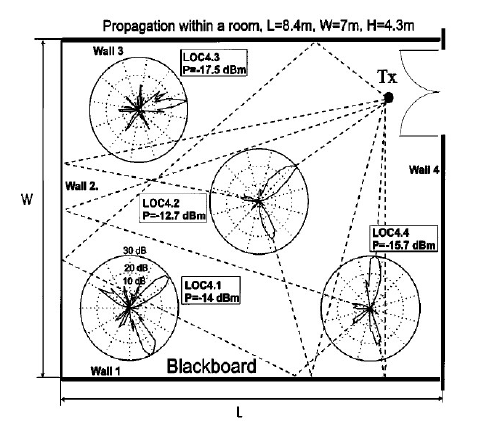
\includegraphics[width=0.8\linewidth]{figs/fig3.1}
    \caption{ Измерение AOA для определения пути распространения в помещении,
        измеренная мощность показана в полярных координатах, $P$ -- максимум
        измеренной мощности. Геометрические лучи показаны только для позиций
        4.2 и 4.4 \cite{Xu2002}.}
    \label{fig:3.1}
\end{figure}

\begin{figure}[h]
    \centering
    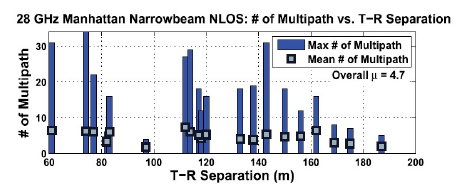
\includegraphics[width=0.8\linewidth]{figs/fig3.2}
    \caption{28 GHz unique antenna azimuth and elevation pointing angle, NLOS
        maximum and mean MPCs as a function of TX-RX separation distance for
        narrow-beam antenna measurements in Manhattan. The overall mean number
        of MPCs over all TX-RX antenna pointing angle combinations and TX-RX
    separation distances is also presented \cite{Rappaport2015}.}
    \label{fig:3.2}
\end{figure}
Basing on the reviewed papers we can conclude that mmWave channel features
allow one to single out several strong propagation paths and determine their
AOAs.

\section{Оценка угла прихода (Angle of arrival estimation)}

Как показано выше, канал миллиметрового диапазона можно представить в виде
набора геометрических лучей.  Самые сильные лучи могут быть
использованы для передачи данных. Как правило, диаграмма направленности
антенны формируется по направлению луча прямой видимости (Line of Sight).
Однако в случае не прямой видимости (Non Line of Sight), может быть
выбран самый сильный отраженный луч. Это причина, почему определение угла
прихода играет ключевую роль в некоторых случаях формирования ДН. Оценка угла
прихода,которая также упоминается в литературе как оценка угла места,
обычно рассматриваемая в задачах радиолокации. Для этих задач уже
разработаны алгоритмы и аппаратные реализации во времена зарождения радиолокации. Эти
алгоритмы совершенствовались, с появлением фазированных антенных решеток.
Этот опыт кажется чрезмерно полезным при наличие аппаратных ограничений систем
связи миллиметрового диапазона при низком количество цифровых портов по сравнению с имеющимся
количеством антенных элементов.  Другой набор алгоритмов пришел из приложений
спектрального анализа. В них обычно предполагается, что сигнал каждой антенны
принимается независимо.  Эти алгоритмы очень эффективны и дают возможность
оценить направления на несколько целей (лучей) одновременно и имеют
сверхразрешение способность. С другой стороны, они
требуют значительных вычислительных ресурсов.
Кроме того, есть некоторые дополнительные специальные методы, такие как
synthesizing a virual aperture, позволяет достигать высокого разрешения и
точности пеленгации. 
В этом разделе мы рассмотрим и систематизируем существующие подходы
к оценке АОА, которые нам удалось найти в открытых литературных источниках.
Будут представлены их преимущества и недостатки.  
На этапе моделирования в следующей части этой работы, мы сократим этот список и
выделим наиболее перспективные методы.

\subsection{Метод Фурье и метод средних периодограмм}

Простейшая алгоритм оценки AOA называется бимформинг \cite{Tuncer2009, Stoica2005}. В
некоторой литературе этот метод также называется метод Фурье \cite{Allen2006}. 
Основная идея заключается в максимизации мощности, принятой с определенного
направления.

Определим сигнал $\vec{y}(t)$ принятой антенной решеткой от некоторого
удаленного источника.

\begin{equation}
    \label{eq:3.1}
    \vec{y}(t) = a(t) \vec{s}(\phi_{src}) + \vec{\xi}(t),
\end{equation}
где ${\vec{s}(\phi_{src})}$ весовой вектор источника сигнала,
$\phi_{src}$ -- угол прихода (AOA); $\vec \xi$ -- вектор шума.
A certain elevent of the steering vector is 
Каждый элемент весового вектора представляется в виде
\begin{equation}
    \qty{\vec{s}(\phi)}_n = \exp{-i(\vec k (\phi), \vec \rho_n)},
\end{equation}
где $\vec k (\phi_{src})$ is n-ый волновой вектор, $\vec\rho_n$ радиус-вектор
n-го элемента антенны. 
В случае эквидистантной антенной решетки (ULA), последнее уравнение приведется
к виде
\begin{equation}
    \qty{\vec s(\phi)}_n = \exp{i2\pi\frac{d}{\lambda}\sin(\phi)n},
\end{equation}
где $d$ -- расстояние между элементами антенной решетки, $\lambda$ -- длина
волны излученного сигнала.

Чтобы получить максимальную мощность с какого-то направления
$\phi$ необходимо сформировать соответствующую диаграмму направленности
(бимформинг). Это делается с использованием так называемого вектора бимформинга
$\vec w (\phi) = \vec s(\phi)/\rVert(\vec s(\phi))\lVert$.

На практике, этот весовой вектор обычно модифицируется окном, выбранным
для подавления уровня боковых лепестков ДН до необходимого уровня. Мы будем
использовать нормированный, но не взвешенный вектор бимформинга, что делает
мощность шума на выходе формирователя луча (принимаемую мощность) такой же, как
на антенне.

Here we use a normalized but nonwindowed weight vector,
which makes the noise power at the beamformer output (received power) the same as at the antenna
elements \cite{Tuncer2009}. 

На основе вектора бимформинга искомая функция будет следующей
\begin{equation}
    p(\phi) = \abs{\vec w^H (\phi) \vec y}^2.
\end{equation}

Физически, функция $p(\phi)$  является мощностью выходного сигнала антенной
решетки. Тогда оценка АОА получается как значение угла
$\phi$, обеспечивающий максимум функции $p(\phi)$.

\begin{equation}
    \phi = argmax~p(\phi)
\end{equation}

\begin{figure}
    \centering
    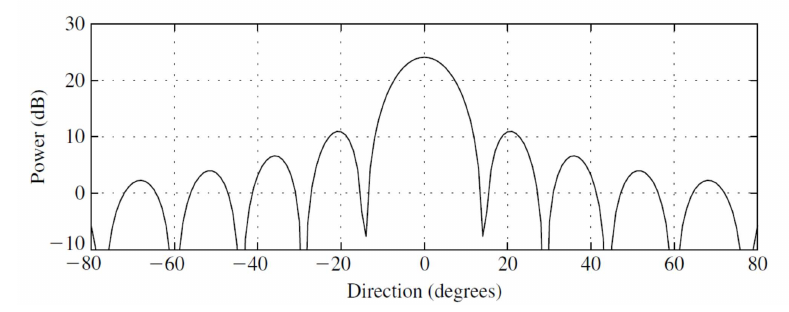
\includegraphics[width=\linewidth]{figs/fig3.9}
    \caption{ДН (невзвещенная) для 16-ти элементной эквидистантной линейной
        решетки ($\frac{d}{\lambda}=0.5$), сформированной на направление 0
        град. \cite{Tuncer2009}. }
    \label{fig:3.9}
\end{figure}

Отметим, что этот алгоритм соответствует обобщенной оценке максимального
правдоподобия в случае модели \eqref{eq:3.1} \cite{Tuncer2009}.

Для фазированной антенной решетки
функция поиска может быть оценена во временной области посредством переключения
луча. Если количество приемников (цифровых портов) равно количеству антенных
элементов, искомая функция $p(\phi)$ может быть оценена в цифровой области \cite{Stoica2005}.
В литературе этот подход также называется методом Бартлетта \cite{Godara2004}. 

Функция $p(\phi)$ примет вид
\begin{equation}
    p(\phi) = \frac{\vec s^H(\varphi) \hat{\vec M} \vec s (\phi)}{N^2},
\end{equation}
где $\hat \vec M$ -- оценка корреляционной матрицы принятого сигнала
\begin{equation}
    \hat {\vec M} = \frac{1}{L} \sum\limits_{t=1}^{L} \vec y(t) y^H (t)
\end{equation}

%As for sidelobe level, it can affect AOA estimation in case of multipath propagation. In order to
%reduce sidelobe level antenna array is weighted with some window function which sets amplitude
%spatial distribution. There are plenty of window functions. The most common of them are Hamming,
%Hanning, Bartlett, Blackman, Chebyshev and Kaiser windows. Note that choice of the window is
%always a trade-off between side lobes level (interference influence) and main lobe width (resolution).
%For example, the Blackman window provides the lowest side lobes level and the widest main lobe.
%Unlike other windows which are fixed, Kaiser and Chebyshev windows provide some flexibility in
%resulting beam pattern properties. The Kaiser window is an approximation of the
%optimal window which maximizes the relative energy in the main lobe
%\cite{Stoica2005}. 
%It is often chosen over the fixed window
%designs because it has a lower sidelobe level when it is selected to have the same main lobe width as
%the corresponding fixed window (or narrower main lobe width for a given sidelobe level). The
%Chebyshev window has the property that the peak level of the sidelobe “ripples” is set constant.
%Under this restriction the window provides the minimal main lobe width. The detailed windows
%description and their comparison analysis can be found in \cite{Stoica2005}
%\cite{Allen2006}. Note, that listed window
%functions can be implemented in hardware via fixed attenuation in waveguides.
%The beamforming based DOA estimation algorithm can be implemented relaying on beam sweep
%procedure used in mm wave communication systems for beam management \cite{Chavva2019}.
%Finally, we can distinguish the following pros and cons of this approach.
Что касается уровня боковых лепестков, то он может повлиять на оценку AOA при многолучевом распространении. Чтобы уменьшить уровень боковых
лепестков антенная решетка взвешивается с некоторой оконной функцией, которая
устанавливает пространственное распределение амплитуды. 
Наиболее распространены окна Хэмминга, Ханнинга, Бартлетта, Блэкмана,
Чебышева и Кайзера. Обратите внимание, что выбор окна всегда компромисс между
уровнем боковых лепестков (влияние помех) и шириной главного лепестка
(разрешение).  Например, окно Блэкмана обеспечивает самый низкий уровень
боковых лепестков и самый широкий главный лепесток.  В отличие от других
фиксированных окон, окна Кайзера и Чебышева обеспечивают некоторую гибкость в
настройке результирующих свойств диаграммы направленности. Окно Кайзера
является аппроксимацией оптимального окна, которое максимизирует относительную
мощность в главном лепестке \cite{Stoica2005}.  Его часто выбирают вместо
фиксированного окна, потому что оно имеет более низкий уровень
боковых лепестков, когда он выбран, чтобы иметь ту же ширину основного
лепестка, что и соответствующее фиксированное окно (или более узкая ширина
основного лепестка для данного уровня бокового лепестка).  Окно Чебышева имеет
то свойство, что пиковый уровень боковых лепестков задается
постоянным.  При этом ограничении окно обеспечивает минимальную ширину главного
лепестка. Подробное описание различных оконных функций и их сравнительный анализ можно найти
в \cite{Stoica2005} \cite{Allen2006}. 
%Обратите внимание, что указанное окно
%функции могут быть реализованы аппаратно через фиксированное затухание в
%волноводах.  Алгоритм оценки DOA на основе формирования луча может быть
%реализован с ретрансляцией по развертке луча.  процедура, используемая в
%системах связи миллиметрового диапазона для управления лучом \cite{Chavva2019}.
%Наконец, можно выделить следующие плюсы и минусы этого подхода.

\paragraph{Преимущества}%
\begin{enumerate}
    \item Теоретически, метод Фурье и метод Бартлетта являются оптимальными
        решениями для оценки AOA в
    случай однолучевого канала.
\end{enumerate}

\paragraph{Недостатки}%

\begin{enumerate}
    %\item In practice, the search accuracy is affected by some adverse factors.
        %First, the derivative of the search function is equal to zero at the
        %extremum point. It leads to “flat” top and makes it difficult to
        %estimate extremum point precisely. Second, it is necessary to provide a
        %high angle discretization rate to provide acceptable AOA estimation
        %accuracy if no additional techniques are used.

    %\item The solution may be not appropriate in case of user mobility if the
        %search is implemented via beam sweeping in time domain.
    %\item The method provides low resolution ability which depends on beam
        %pattern’s main lobe
    %width. Increasing of SNR or evaluation time does not lead to enhancement of resolution
    %quality. That makes this approach hardly matched for multipath AOA estimation.
    %\item In case of close multipath AOA estimation there is significant bias of
        %direction (systematic error).
\item На практике, точность поиска снижается из-за некоторых факторов.
    Во-первых, производная функции $p(\phi)$ равна нулю в
         точка экстремума. Это приводит к «плоской» вершине и затрудняет точное
         определение точки экстремума. Во-вторых, необходимо обеспечить
         высокую дискретизацию по углу для обеспечения приемлемой оценки.
     \item Решение может не подойти в случае достаточно мобильных пользователей, если
         поиск реализован с помощью сканирования во временной области.
     \item Метод обеспечивает разрешающую способность, зависящую
         от ширина главного лепестка ДН. Увеличение SNR или времени
         сканирования не приводит к качественному улучшению разрешения.  Это делает
         этот подход малопригодным для оценки многолучевого АОА.
     \item В случае нескольких близко расположенных АОА наблюдается
         значительно смещение оценки (систематическая ошибка).
\end{enumerate}


\subsection{Метод максимального правдоподобия}%
\label{sub:metod_maksimal_nogo_pravdopodobiia}
При наличии нескольких путей распространения, оптимальная оценка AOA может быть
получена с помощью максимально правдоподовной оценки (MLE).
 \cite{Tuncer2009}. Соответствующая модель сигнала:
\begin{equation}
    \label{eq:3.8}
    \vec y(t) = \sum\limits_{q=1}^{J} a_q(t)\vec s(\phi_q) + \vec \xi(t),
\end{equation}
где $J$ число путей распространения; $a_q(t)$ -- комплексная амплитуда q-то
луча, $\vec s(\phi_q)$ весовой вектор;  $\phi_q$ -- угол прихода (AOA) q-то
луча и $\xi(t)$ -- вектор белого гауссового шума. 
Для этой модели канала критерий МП может быть записан как критерий минимума
среднеквадратичной ошибки (MMSE)
 \begin{equation}
    \label{eq:}
    d(\phi_1, \hdots, \phi_J) = \sum\limits_{t}^{} \abs{\vec(t) -
    \sum\limits_{q=1}^{J} a_q(t) \vec s(\phi_q)}^2 \to_{\phi_q} min
\end{equation}
Это уравнение может быть представлено в виде
\begin{equation}
    \label{eq:}
    d(\phi_1, \hdots, \phi_J) = \sum\limits_{t}^{} \vec y^H(t) \vec
P_\perp(\phi_1, \hdots, \phi_J) \vec y(t) \to_{\phi_q} min
\end{equation}

\begin{equation}
    \label{eq:}
    \vec P_\perp(\phi_1, \hdots, \phi_J) = \vec E - \vec S(\vec S^H \vec S)^{-1}
    \vec S^H,
\end{equation}
where $\vec P_\perp$ is a projection matrix and  $\vec S = \qty[\vec s(\phi_1)
\dots \vec s (\phi_J)]$. The minimization of  $d(\phi_1, \hdots, \phi_J)$
needs to be numerical. 
It is generally computationally intensive and require J-dimensional search. In
general a “brute-force” search over a selected grid of values of $(\phi_1,
\hdots, \phi_J)$ is necessary, followed by
interpolation in the neighborhood of the minimum point to compute the final estimate.

\begin{figure}[h]
    \centering
    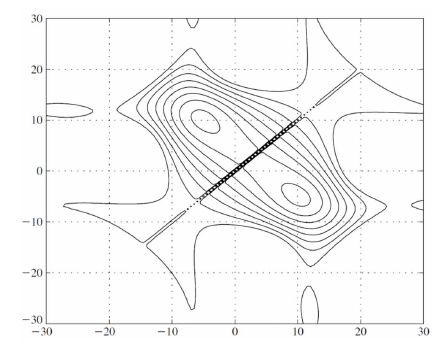
\includegraphics[width=0.6\linewidth]{figs/fig3.10}
    \caption{Maximum likelihood cost function (3.11) for an 8-elemennt ULA and
    two emitters at $\phi_1=-5^\circ$ and  $\phi_2 = 10^\circ$ \cite{Tuncer2009}}
    \label{fig:3.10}
\end{figure}

Finally, we can distinguish the following pros and cons of this approach.
\paragraph{Advantages}%
\label{par:advantages}
\begin{enumerate}
    \item ML estimator provides the optimal solution in case of multiple dominant propagation paths
(AOAs).
\end{enumerate}

\paragraph{Disadvantages}%
\label{par:disadvantages}
\begin{enumerate}
     \item Digital antenna array is required
     \item Excessively high computational cost (“brute force” search).
     \item Maximum likelihood function does not allow one to estimate the number of AOAs. If the
    number of the propagation paths is not known, the method is not optimal.
(AOAs).
\end{enumerate}


\subsection{Monopulse}%
\label{sub:monopulse}

A variation of the beamformer involves a method, often referred to as
monopulse, commonly used in radar systems for target tracking. This method
involves taking the difference between the outputs of two beams pointing in
slightly different directions \cite{Tuncer2009}. The search function is the following
\begin{equation}
    \label{eq:}
    b(\phi) = \frac{1}{\Delta} \qty(\abs{\vec w^H(\phi+0.5 \Delta)\vec y}^2)
    -
    \qty(\abs{\vec w^H(\phi-0.5 \Delta)\vec y}^2) \approx \dv{p(\phi)}{\phi} ,
\end{equation}
where $p(\phi)$ and  $\vec w(\phi)$ are defined as in section 3.2.1. 
The estimation of AOA is obtained as the
value of angle $\phi$ which provides zero search function value
\begin{equation}
    \label{eq:}
    \phi = arg\qty{b(\phi) = 0}.
\end{equation}

In fact, $\Delta$ can be on the order of one beamwidth and $b(\phi)$ will still
be well approximated by derivative of $p(\phi)$ because $b(\phi)$ is nearly
linear over a significant range of angles around the zero- response point
\cite{Tuncer2009}.
This property of the search function gives the opportunity to decrease the
angle discretization rate and apply linear approximation to find AOA. Note,
that this approach is often used together with a rough classical beamforming
method that determines an angle range to accurate search.  An additional
feature of this algorithm is that the output is positive if the emitter is to
the right of the direction in which the difference beam is pointed and negative
if it is to the left. This ability to determine the direction of the emitter
relative to the pointing direction by the sign of the response is useful in
tracking applications \cite{Tuncer2009}.

\begin{figure}[h]
    \centering
    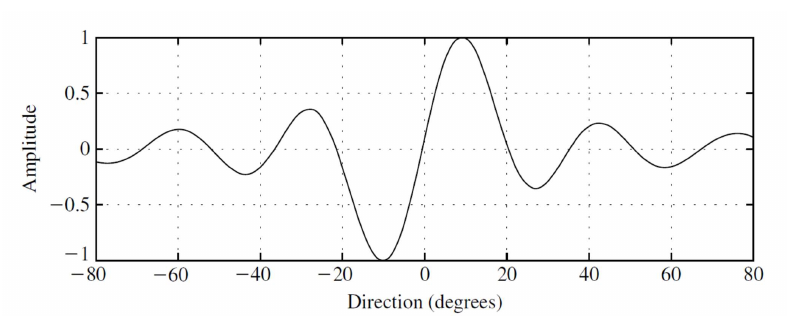
\includegraphics[width=\linewidth]{figs/fig3.11}
    \caption{Response of a monopulse system for 16-element ULA \cite{Tuncer2009}. Source
    direction is 0 deg.}
    \label{fig:3.11}
\end{figure}
Another variant of the algorithm is often called Monopulse Ratio or Amplitude
Comparison Monopulse \cite{Mosca1969}. This algorithm requires coherent reception with two
channels (RF-chains): sum and difference. The sum channel is formed with beam
pattern which has a maximum for a certain direction. The difference beam
pattern has a null for this direction. In \cite{Kim2018} the algorithm which uses TDM for
sum and difference channels is proposed and investigated. It employs cycle
prefix of OFDM signal to receive two identical signals with different beam
patterns using a single RF-chain and phased antenna array. This approach seems
promising, but there are some issues related to phase shifter switching delay
and multipath propagation influence.
The metric of monopulse ratio is \cite{Kim2018}
\begin{equation}
    \label{eq:}
    \tan(\frac{N}{4}(\phi_{src} - \phi)) = 
    \frac{Im\qty{\sum\limits_{k} y_d(k) y_s^*(k)}}{\sum\limits_{k}
    \abs{y_s(k)}^2},
\end{equation}
where $\phi_{src}$ is actual  AOA;  $\phi$ is roughly estimated AOA via beam
sweeping (it is the direction of the sum beam); N is number of antenna
elements; $y_s(k)$ and  $y_d(k)$ are signals f the sum and difference channels
respectively.
 \begin{equation}
    \label{eq:}
    y_s(t) = a(t) \vec w_s^H \vec s(\phi_{src}) + \vec w_s^H \vec \xi(t)
\end{equation}
 \begin{equation}
    \label{eq:}
    y_d(t) = a(t) \vec w_d^H \vec s(\phi_{src}) + \vec w_d^H \vec \xi(t)
\end{equation}

For a linear antenna array the corresponding beamforming vectors are
\begin{equation}
    \label{eq:}
    \qty{\vec w_s (\phi)}_n = \exp{i_2\pi \frac{d}{\lambda}} \sin \phi
\end{equation}
\begin{equation}
    \label{eq:}
    \qty{\vec w_d (\phi)}_{n < \frac n {N}{2}} = - \exp{i_2\pi n \frac{d}{\lambda}} \sin \phi
\end{equation}
\begin{equation}
    \label{eq:}
    \qty{\vec w_d(\phi)}_{n\geq \frac{N}{2}} = +\exp{i2\pi \frac{d}{\lambda}
    \sin \phi (n - 0.5N)},
\end{equation}

\begin{figure}[htpb]
    \centering
    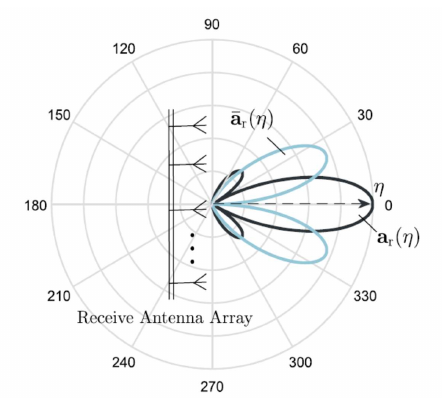
\includegraphics[width=0.6\linewidth]{figs/fig3.12}
    \caption{Sum and difference beam patterns for monopulse ratio algorithm
    \cite{Zhu2016}}
    \label{fig:}
\end{figure}

Monopulse ratio is typically used to estimate a single AOA or resolvable angles
(far spaced targets which are not located within the same beam). However, there
are some modifications that use a complex monopulse ratio and allow one to
detect the multiple targets in a certain beam and estimate their angle
positions \cite{Luoshengbin2016} \cite{Sherman2011}.  As monopulse ratio requires a coherent signal reception
using two channels with different beam patterns it is hardly appropriate for
simple mm-wave system design which consists of only a single RF-chain and can
set only predefined Fourier codebook beams. In \cite{Zhu2016} auxiliary beam approach is
proposed which is similar to monopulse ratio. The principle difference consists
of two points. Firstly, the auxiliary beam approach employs simple beams with a
single main lobe as well as the original monopulse approach does. Secondly, it
employs incoherent signal receptions for different beams and can be implemented
using a single RF-chain.

\begin{equation}
    \label{eq:}
    \zeta_n = \frac{p(\eta_n - \delta) - p(\eta_n + \delta)}{p(\eta_n - \delta)
    + p(\eta_n + \delta)} = 
    \frac{\sin(\psi - \eta_n)\sin\delta}{1 - \cos(\psi - \eta_n)\cos \delta}
\end{equation}

\begin{equation}
    \label{eq:}
    \psi = \eta_n - \arcsin( 
    \zeta_n \frac{\sin\delta}{\sin^2 \delta + \zeta^2_n \cos^2\delta}
    -
    \frac{\zeta_n \sqrt{1-\zeta^2_n} \sin \delta \cos \delta}{\sin^2\delta +
    \zeta^2_n \cos^2 \delta}
    )
\end{equation}
where $\psi_n = 2\pi \frac{d}{\lambda} \sin \phi$ is a spatial frequency for
beam with mainlobe direction angle $\phi$; $\eta$ is a central spatial
frequency for auxiliary beams pair; $n$ is the best auxiliary beams pair index;
$\delta = \frac{\pi}{N}$; $N$ is a number of antenna elements; $p(\eta)$ is
power of received signal for beam with spatial frequency $\eta$.

\begin{figure}[h]
    \centering
    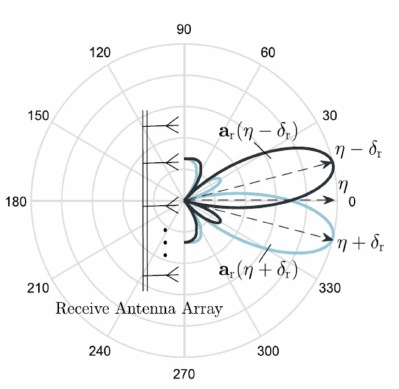
\includegraphics[width=0.6\linewidth]{figs/fig3.13}
    \caption{Auxiliary beam approach patterns \cite{Zhu2016}}
    \label{fig:}
\end{figure}

It is noted in \cite{Sherman2011} that described auxiliary beam approach can provide wrong
result if AOA is near direction of some auxiliary beam and SNR is low, because
it can lead to error in pair selection. In \cite{Sherman2011} it is proposed to employ
additional two beams in this case with the aim to overcome the problem.

\begin{figure}[h]
    \centering
    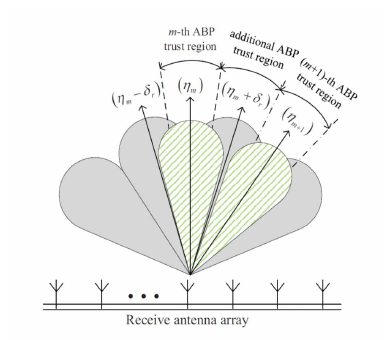
\includegraphics[width=0.6\linewidth]{figs/fig3.14}
    \caption{Auxiliary beam approach and additional auxiliary beam pair
    \cite{Tuncer2009}}
    \label{fig:}
\end{figure}

Finally, we can distinguish the following pros and cons of this approach.
\paragraph{Преимущества}%
\label{par:preimushchestva}

\begin{enumerate}
    \item In practice, it is more convenient and precise than beamforming
        method because the search function is quite steep in the area near AOA.
    \item It can be implemented using phased antenna array with single digital
        port (enable low hardware cost).
    \item Relatively low number of beams is necessary to evaluate AOA.
    \item It potentially could be used together with beam tracking algorithms.
    \item Multiple path AOAs estimation is potentially available using complex
        monopulse ratio.
\end{enumerate}

\paragraph{Недостатки}%
\label{par:nedostatki}
\begin{enumerate}
    \item As a variation of beamforming approach the original method provides
        low resolution ability which depends on beam pattern main lobe width.
        Increasing SNR or evaluation time does not lead to enhancement of
        resolution quality. The high resolution can be achieved using a
        coherent signal reception and complex multipath ratio only.
    \item In case of close multipath AOA estimation, significant bias of
        direction (systematic error) is possible.
\end{enumerate}

\subsection{Minimum variance distortionless response estimator (Capon method)}%
\label{sub:minimum_variance_distortionless_response_estimator_capon_method_}

Another approach similar to beamforming method is Minimum Variance
Distortionless Response Estimator (MVDR) which is also referred to as Capon
method \cite{Stoica2005,Allen2006, Godara2004}. The main idea of this approach is to form beamforming
vector $\vec w(\phi)$  to minimize signal power received from all directions (total
received power) under constant gain for some direction $\phi$.

\begin{figure}[h]
    \centering
    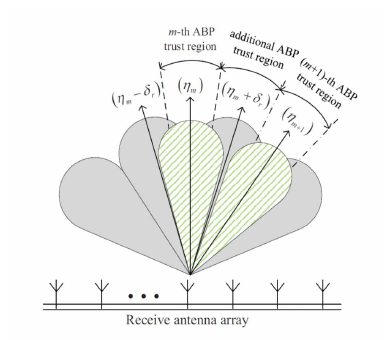
\includegraphics[width=0.6\linewidth]{figs/fig3.14.png}
    \caption{The base idea of Capon method}
    \label{fig:3.15}
\end{figure}
The beamforming vector in this case is obtained as a solution of nonlinear
programming task \cite{Stoica2005, Godara2004}.

\begin{equation}
    \label{eq:}
    \vec w(\phi) = \frac{\hat \vec M^{-1} \vec s (\phi)}{\vec s^H(\phi)\hat
    \vec M^{-1} \vec s(\phi)},
\end{equation}
where $s(\phi)$ is a steering vector defined in (3.2) and $\vec \hat M$ is an estimated signal correlation matrix (3.7).
That leads to the following search function:
\begin{equation}
    \label{eq:}
    p(\phi) = \frac{1}{s^H(\phi) \vec M^{-1} \vec s(\phi)}
\end{equation}
The function represents the received power. The peaks of this function
correspond to AOAs of propagation paths. The resolution of the method increases
with SNR.

For this method we can distinguish the following pros and cons.
\paragraph{Преимущества}%
\label{par:preimushchestva}
\begin{enumerate}
 \item Capon method provides high AOA estimation accuracy.
 \item The method can be used for multiple AOAs evaluation. It provides
     superresolution ability.
 \item It can be implemented in the hardware as the search function has a
     physical meaning of received power.

\end{enumerate}
\paragraph{Недостатки}%
\label{par:nedostatki}

\begin{enumerate}
 \item The resolution is limited even the correlation matrix M is known
     precisely. If one desires to improve the potential resolution, it is
     necessary to increase SNR or the number of antenna elements.
 \item Matrix inversion used in the method has high computational cost.
\end{enumerate}













